\chapter{اللدونة العصبية، والتعلم، والذاكرة}\label{ch:b3:learning-memory}

في عام 1953 استأصل جرّاح الجزء الداخلي من الفصّين الصدغيين
كليهما عند شاب مصاب بصرع عصيّ. فخفّت النوبات؛ وأما المريض،
الذي عُرف خمسين سنة بالحرفين H.M.، فلم يكوّن بعدها ذاكرة
دائمة لأي حدث. كان يقدر على إدارة محادثة، وعلى أن يتعلم رسم
نجمة في مرآة كأي إنسان --- وأن ينكر كل يوم أنه رأى المهمة
قط --- وكان يذكر طفولته. فتبيّن أن الذاكرة ليست شيئًا
واحدًا، وأن تكوين ذكريات جديدة للأحداث يتوقف على بنية بحجم
الإبهام. وما الذي يتغير في دماغ حين يتعلم هو أقدم أسئلة علم
الأعصاب، وجوابه، الذي استُخرج في بزّاقة بحر فيها عشرون ألف
عصبون وفي شرائح من \omterm{def:b3:learning-memory:kinds}{حُصين} الجرذ، هو أن المشابك تغيّر قوتها
بحسب ما يمر بها --- وهي قاعدة حدسها دونالد هِب عام 1949
وتبيّن أن جزيئًا، هو \omterm{prop:b3:learning-memory:nmda}{مستقبل NMDA}، ينفّذها. ويتناول هذا الفصل
تلك القاعدة وآلتها، والدارات التي تستعملها لتخزين الأماكن
والأحداث، والرياضيات التي تقول ما يقدر جهاز كهذا على تعلمه
وكم يسع، وإشارة المكافأة التي تخبره بما يستحق التعلم.

\section{أضرب الذاكرة وأين تسكن}

\begin{definition}[صور التعلم والذاكرة]\label{def:b3:learning-memory:kinds}
\index{تعوّد}\index{تحسيس}\index{إشراط}\index{ذاكرة تصريحية}\index{ذاكرة إجرائية}\index{ترسيخ}\index{حُصين}
أبسط التعلم \emph{غير ترابطي}: و\emph{التعوّد} استجابة
هابطة لمنبّه غير ضار متكرر، و\emph{التحسيس} استجابة معزَّزة
بعد منبّه ضار. والتعلم \emph{الترابطي} يربط حدثين: ففي
\emph{الإشراط الكلاسيكي} (بافلوف) يصير منبّه محايد يتنبأ
بمكافأة أو بعقاب مستدعيًا للاستجابة؛ وفي \emph{الإشراط
الإجرائي} يتكرر فعل يُكافَأ. وتنقسم ذاكرة الإنسان إلى ذاكرة
\emph{تصريحية} --- للوقائع والأحداث، تُستدعى واعيةً، وتتوقف
على \emph{الحُصين} والفصّ الصدغي الإنسي --- وذاكرة \emph{غير
تصريحية} --- للمهارات والعادات (المخطط، \omterm{def:b3:nervous-systems:plan}{والمخيخ})، وللخوف
المشروط (اللوزة)، وللتهيئة (القشرة) --- تُعبَّر عنها في
الأداء بلا استذكار. وتُحفظ الذكرى أولًا في صورة قصيرة الأمد
هشّة، تدوم ثوانيَ إلى ساعات، ثم \emph{تُرسَّخ} على مدى ساعات
إلى سنين في صورة مستقرة طويلة الأمد لا تعود تحتاج إلى
الحُصين وتقيم في القشرة.
\end{definition}

\begin{proof}[شواهد]
أبلغ سكوفيل وميلنر (1957) عن H.M.: فبعد استئصال الحُصينين
كليهما والقشرة المجاورة، بقي ذكاؤه وذكرياته السابقة للعملية
سليمة في معظمها، وبقيت ذاكرته العاملة سوية ما دام منتبهًا
إلى شيء، غير أنه لم يعد يقدر على تكوين ذكرى لأي حدث أو
واقعة. وقد تعلم مهارات حركية بمعدل سويّ على مدى أيام وهو
ينكر أنه تمرّن --- فذاكرة المهارة لم تحتج إلى \omterm{def:b3:learning-memory:kinds}{الحُصين} ---
وكان يذكر الماضي البعيد أفضل من السنوات التي سبقت الجراحة
مباشرةً، \omterm{def:b3:learning-memory:kinds}{فالحُصين} إذن لازم لوضع الذكريات التصريحية ولحفظها
حينًا، لا لتخزينها إلى الأبد. وأظهرت قردة وجرذان بآفات
مماثلة الانفصال نفسه، فأعادت دراسة مريض واحد تنظيم الحقل
كله.
\end{proof}

\section{قاعدة هِب وجزيئها}

\begin{definition}[اللدونة الهِبّية، والتقوية والاكتئاب طويلا الأمد]\label{def:b3:learning-memory:ltp}
\index{قاعدة هِب}\index{تقوية طويلة الأمد}\index{اكتئاب طويل الأمد}\index{لدونة معتمدة على توقيت الشوكات}
اقترح هِب (1949) أن العصبون قبل المشبكي حين يشارك مرارًا في
إشعال العصبون بعد المشبكي تتقوى الوصلة بينهما --- ``الخلايا
التي تشتعل معًا تتصل معًا''. و\emph{التقوية طويلة الأمد}
(LTP) هي صورتها التجريبية: فدفقة قصيرة من تنبيه عالي التردد
لسبيل ما تترك المشابك التي فعّلتها أقوى ساعات في شريحة
وأسابيع في حيوان. والتقوية طويلة الأمد \emph{نوعية الدخل}
(فلا تتغير إلا المشابك المنبَّهة)، و\emph{ترابطية} (فدخل
ضعيف مقترن بدخل قوي إلى الخلية نفسها يُقوَّى)، وتحتاج إلى
\emph{تعاون} بين الدخلات لإزالة استقطاب الخلية.
و\emph{الاكتئاب طويل الأمد} (LTD) نقيضها، ينتجه نشاط مطوَّل
منخفض التردد. وفي \emph{اللدونة المعتمدة على توقيت الشوكات}
يحدد الترتيبُ الإشارةَ: فشوكة قبل مشبكية تسبق بضعة ميلي
ثوانٍ الشوكة بعد المشبكية \emph{قبلها} تقوّي المشبك، وواحدة
\emph{بعدها} تضعفه، ضمن نافذة قدرها نحو \qty{20}{ms} في كل
جهة --- فالمشبك يتعلم أن يتنبأ، لا أن يترابط فحسب.
\end{definition}

\begin{proposition}[مستقبل NMDA كاشفًا للتزامن]\label{prop:b3:learning-memory:nmda}
\index{مستقبل NMDA}\index{مستقبل AMPA}\index{CaMKII}\index{CREB}\index{شوكة تغصنية}
عند المشابك المهيِّجة يعمل الغلوتامات على مستقبلين. فمستقبل
\emph{AMPA} ينفتح عند الارتباط ويحمل التيار المشبكي
الاعتيادي. وأما مستقبل \emph{NMDA} فيربط الغلوتامات لكنه
محجوب عند كمون الراحة بأيون مغنيزيوم في مساميه؛ ولا يُطرد
المغنيزيوم وتنقل القناة إلا حين يزول استقطاب الغشاء بعد
المشبكي --- بدخلات كثيرة دفعة واحدة، أو بكمون عمل راجع ---
فيدخل الكالسيوم. \omterm{prop:b3:learning-memory:nmda}{فمستقبل NMDA} إذن لا ينفتح إلا حين يتزامن
الإطلاق قبل المشبكي (الغلوتامات) مع النشاط بعد المشبكي
(زوال الاستقطاب): فهو بوابة ``و'' عند هِب في بروتين واحد.
والكالسيوم الداخل إلى \emph{\omterm{prop:b3:learning-memory:nmda}{شوكة تغصنية}} يفعّل الكيناز
\emph{CaMKII}، الذي يفسفر مستقبلات AMPA ويسوق مزيدًا منها
إلى المشبك من احتياطي --- فيصير المشبك أقوى في دقائق
(التقوية المبكرة). وأما ارتفاع الكالسيوم الكبير البطيء
فيفعّل بدل ذلك الفسفاتاز كالسينورين، الذي يزيل مستقبلات
AMPA: وذلك \omterm{def:b3:learning-memory:ltp}{الاكتئاب طويل الأمد}. والتقوية التي تدوم أكثر من
بضع ساعات (التقوية المتأخرة) تحتاج إلى بروتين جديد: فتبلغ
الكينازات النواة، ويشغّل عامل الاستنساخ \emph{CREB}
مورّثات، وتنمو الشوكة وقد تنقسم --- وهو الاشتراط نفسه على
التعبير المورّثي الذي يفصل الذاكرة القصيرة الأمد عن الطويلة
في كل حيوان دُرس.
\end{proposition}

\begin{proof}[شواهد]
نبّه بليس ولومو (1973) السبيل المثقوب الداخل إلى \omterm{def:b3:learning-memory:kinds}{حُصين}
الأرنب بقطار من النبضات فوجدا الاستجابة المستثارة متضخمة
ساعات بعد ذلك --- وتلك أول \omterm{def:b3:learning-memory:ltp}{تقوية طويلة الأمد}. وبيّن
كولينغريدج (1983) أن حاجبًا \omterm{prop:b3:learning-memory:nmda}{لمستقبل NMDA} (وهو AP5) يمنع
استحداث التقوية لا الاستجابة المشبكية الاعتيادية؛ وحقن
موريس (1986) AP5 في \omterm{def:b3:learning-memory:kinds}{حُصين} جرذان فوجد أنها لم تعد تقدر على
تعلم موضع منصة مخبأة في حوض ماء مع أنها تسبح وترى سويًّا؛
والفئران التي حُذف فيها \omterm{prop:b3:learning-memory:nmda}{مستقبل NMDA} في منطقة \omterm{def:b3:learning-memory:hippocampus}{CA1} من \omterm{def:b3:learning-memory:kinds}{الحُصين}
وحدها افتقرت إلى التقوية هناك وإلى الذاكرة المكانية معًا.
فالمستقبل نفسه، في الموضع نفسه، كان لازمًا للتغير المشبكي
وللتعلم.
\end{proof}

\begin{omfigure}
\begin{tikzpicture}[every node/.style={font=\scriptsize}, >=stealth]
  % presynaptic terminal
  \draw[thick, omDef, fill=omDef!12] (0,2.2) .. controls (0,3.4) and (4,3.4) .. (4,2.2) -- (4,1.7) -- (0,1.7) -- cycle;
  \node at (2,2.8) {النهاية قبل المشبكية};
  \foreach \p in {(0.8,2.0),(1.6,2.1),(2.6,2.0),(3.3,2.1)} \draw[thick, fill=omDef!40] \p circle (0.17);
  \foreach \p in {(1.2,1.45),(2.0,1.5),(2.9,1.42)} \fill[omProp] \p circle (0.06);
  \node[right, omProp] at (3.3,1.45) {غلوتامات};
  % postsynaptic spine
  \draw[thick, omMeth!70!black, fill=omMeth!10] (-0.6,1.1) -- (4.4,1.1) -- (4.4,-1.2) -- (-0.6,-1.2) -- cycle;
  \node at (0.6,-0.9) {شوكة تغصنية};
  % AMPA
  \draw[thick, fill=omMeth!45] (0.2,0.85) rectangle (0.6,1.35); \node[below, align=center] at (0.1,0.8) {AMPA:\\دخول Na$^{+}$};
  \draw[->, thick] (0.4,1.7) -- (0.4,0.95);
  % NMDA with Mg
  \draw[thick, fill=omThm!35] (2.4,0.85) rectangle (2.9,1.35); \fill[gray!70] (2.65,1.1) circle (0.09); \node[right, font=\tiny] at (2.95,1.1) {حجب Mg$^{2+}$};
  \node[below, align=center] at (2.65,0.8) {NMDA: يحتاج إلى الغلوتامات\\\emph{و}إلى زوال الاستقطاب};
  \draw[->, thick, omThm] (2.65,0.15) -- (2.65,-0.5) node[below] {Ca$^{2+}$};
  % downstream
  \node[draw, rounded corners, fill=omThm!15, font=\tiny] (cam) at (5.6,0.3) {CaMKII};
  \draw[->, thick] (2.9,-0.5) -- (cam);
  \node[draw, rounded corners, fill=omMeth!25, font=\tiny, align=center] (ampa) at (8.2,1.0) {إدخال مزيد من مستقبلات AMPA:\\تقوية مبكرة (دقائق)};
  \node[draw, rounded corners, fill=omMeth!25, font=\tiny, align=center] (creb) at (8.2,-0.5) {CREB، وبروتينات جديدة،\\ونمو الشوكة: تقوية متأخرة (ساعات فأكثر)};
  \draw[->, thick] (cam) -- (ampa.west); \draw[->, thick] (cam) -- (creb.west);
  \node[draw, rounded corners, fill=omDef!15, font=\tiny, align=center] (ltd) at (8.2,-1.8) {ارتفاع Ca$^{2+}$ بطيء صغير: كالسينورين،\\وإزالة AMPA: اكتئاب};
  \draw[->, thick, dashed] (2.9,-0.7) .. controls (4.5,-1.6) .. (ltd.west);
\end{tikzpicture}

{\small \omterm{prop:b3:learning-memory:nmda}{مستقبل NMDA} بوابةً لهِب. فالغلوتامات وحده يفتح
مستقبلات AMPA؛ وأما قناة NMDA فلا تنقل إلا حين تكون الشوكة
زائلة الاستقطاب أيضًا ويغادر مغنيزيومُها. والكالسيوم الداخل
عندئذ يحدد مستقبل المشبك: فارتفاع سريع كبير يقويه، وارتفاع
بطيء صغير يضعفه.}
\end{omfigure}

\begin{omfigure}
\begin{tikzpicture}
\begin{axis}[
  width=6.6cm, height=5.2cm,
  axis x line=bottom, axis y line=left,
  xmin=-20, xmax=120, ymin=0, ymax=220,
  xlabel={دقائق}, ylabel={الاستجابة المشبكية (\%)},
  xlabel style={font=\small, at={(axis description cs:0.5,-0.12)}, anchor=north}, ylabel style={font=\small},
  tick label style={font=\scriptsize}, xtick={0,30,60,90,120}, ytick={0,100,200},
  clip=false,
]
\addplot[only marks, mark=*, mark size=1pt, omDef] coordinates {(-18,100) (-15,98) (-12,102) (-9,99) (-6,101) (-3,100) (2,195) (5,180) (8,172) (11,168) (15,165) (20,162) (30,160) (40,158) (50,157) (60,156) (70,156) (80,155) (90,155) (100,154) (110,154) (120,154)};
\addplot[only marks, mark=o, mark size=1pt, gray] coordinates {(-18,100) (-12,101) (-6,99) (2,102) (8,100) (15,101) (30,100) (45,99) (60,101) (75,100) (90,100) (105,101) (120,100)};
\draw[->, thick, omThm] (axis cs:0,215) -- (axis cs:0,200); \node[font=\scriptsize, omThm, anchor=south] at (axis cs:0,216) {كزاز};
\node[font=\scriptsize, omDef, anchor=south west] at (axis cs:35,168) {السبيل المنبَّه: تقوية};
\node[font=\scriptsize, gray, anchor=north west] at (axis cs:35,95) {سبيل الشاهد: بلا تغيّر};
\end{axis}
\begin{axis}[
  at={(7.6cm,0)}, anchor=south west,
  width=6.6cm, height=5.2cm,
  axis x line=middle, axis y line=middle,
  xmin=-60, xmax=60, ymin=-60, ymax=100,
  xlabel={$t_{\text{pre}} - t_{\text{post}}$ (ms)}, ylabel={$\Delta w$ (\%)},
  xlabel style={font=\small, at={(axis description cs:0.5,-0.06)}, anchor=north}, ylabel style={font=\small, at={(axis description cs:0.5,1.02)}, anchor=south},
  tick label style={font=\scriptsize}, xtick={-40,-20,20,40}, ytick={-40,40,80},
  clip=false,
]
\addplot[very thick, omMeth!70!black, domain=-60:-0.5, samples=60] {80*exp(x/15)};
\addplot[very thick, omThm, domain=0.5:60, samples=60] {-45*exp(-x/25)};
\node[font=\scriptsize, omMeth!70!black, anchor=south east] at (axis cs:-8,62) {قبل المشبكية تسبق: تقوية};
\node[font=\scriptsize, omThm, anchor=north west] at (axis cs:8,-22) {بعد المشبكية تسبق: اكتئاب};
\end{axis}
\end{tikzpicture}

{\small يسارًا: \omterm{def:b3:learning-memory:ltp}{التقوية طويلة الأمد} --- بعد كزاز قصير تبقى
استجابة السبيل المنبَّه متضخمة ساعات بينما لا يتغير سبيل غير
منبَّه إلى الخلايا نفسها (نوعية الدخل). ويمينًا: نافذة توقيت
الشوكات --- يتقوى المشبك إن تقدمت الشوكة قبل المشبكية
ويضعف إن تأخرت.}
\end{omfigure}

\begin{theorem}[ما يتعلمه مشبك هِبّي]\label{thm:b3:learning-memory:hebb}
\index{تعلم هِبّي!المركّبة الرئيسة}\index{قاعدة أويا}
ليتلقَّ عصبون دخلات $\mathbf{x} = (x_{1},\dots,x_{n})$ عبر
أوزان $\mathbf{w}$ وليستجب خطيًا، $y = \mathbf{w}\cdot\mathbf{x}$.
\omterm{def:b3:learning-memory:ltp}{فقاعدة هِب}، $\Delta\mathbf{w} = \eta\, y\,\mathbf{x}$، تعطي وسطيًا
على الدخلات
\[
\langle\Delta\mathbf{w}\rangle = \eta\,C\,\mathbf{w}, \qquad C =
\langle\mathbf{x}\mathbf{x}^{\mathsf{T}}\rangle ,
\]
حيث $C$ مصفوفة ترابط الدخلات. فتنمو الأوزان بلا حد، وتنمو
أسرع ما تنمو على امتداد المتجه الذاتي للمصفوفة $C$ ذي أكبر
قيمة ذاتية: فيصير المشبك كاشفًا لنمط الدخل الأكثر حضورًا
--- أي \emph{المركّبة الرئيسة} لدخلاته. ومع حد يعاقب الأوزان
الكبيرة، وهو \emph{\omterm{thm:b3:learning-memory:hebb}{قاعدة أويا}}
$\Delta\mathbf{w} = \eta\, y\,(\mathbf{x} - y\,\mathbf{w})$، يتقارب متجه
الأوزان إلى ذلك المتجه الذاتي معيَّرًا إلى طول الوحدة،
ويصير العصبون كاشفًا مستقرًا للترابط المهيمن فيما يراه.
\end{theorem}
\begin{proof}
بتعويض $y = \mathbf{w}\cdot\mathbf{x} = \mathbf{x}^{\mathsf{T}}
\mathbf{w}$ في \omterm{def:b3:learning-memory:ltp}{قاعدة هِب} نجد $\Delta\mathbf{w} = \eta\,\mathbf{x}
\mathbf{x}^{\mathsf{T}}\mathbf{w}$، ووسطيها على الدخلات (مع
تغيّر $\mathbf{w}$ ببطء) هو $\eta C\mathbf{w}$. والمصفوفة $C$ متناظرة
وشبه معرَّفة موجبًا، فلها متجهات ذاتية متعامدة $\mathbf{e}_{k}$
بقيم ذاتية $\lambda_{k} \ge 0$؛ وبكتابة $\mathbf{w} = \sum_{k}
a_{k}\mathbf{e}_{k}$، تخضع كل مركّبة للعلاقة $\Delta a_{k} = \eta\lambda_{k}
a_{k}$ وتنمو بالمقدار $(1 + \eta\lambda_{k})^{t}$، فتصير المركّبة على
امتداد أكبر قيمة ذاتية مهيمنة على اتجاه $\mathbf{w}$
بينما يتباعد طوله. \omterm{thm:b3:learning-memory:hebb}{وقاعدة أويا} وسطيها $\eta(C\mathbf{w} -
(\mathbf{w}^{\mathsf{T}}C\mathbf{w})\mathbf{w})$؛ وعند نقطة ثابتة
يكون $C\mathbf{w} = (\mathbf{w}^{\mathsf{T}}C\mathbf{w})\mathbf{w}$، فيكون
$\mathbf{w}$ متجهًا ذاتيًا عند $\lambda = \mathbf{w}^{\mathsf{T}}
C\mathbf{w} = \lambda|\mathbf{w}|^{2}$، ومن ثم $|\mathbf{w}| = 1$؛
والنقطة الثابتة على امتداد أكبر قيمة ذاتية هي المستقرة
(إذ يتقلص اضطراب نحو متجه ذاتي آخر، لأن قيمته الذاتية
أصغر)، وذلك مُسلَّم به هنا.
\end{proof}

\begin{example}[دخلان]\label{ex:b3:learning-memory:two-inputs}
يتلقى عصبون دخلين يكونان عادةً فعالين معًا، فتكون $C =
\begin{pmatrix} 1 & 0.8 \\ 0.8 & 1\end{pmatrix}$. والمتجهان الذاتيان هما
$(1,1)/\sqrt{2}$ بقيمة ذاتية $1.8$ و$(1,-1)/\sqrt{2}$ بقيمة
ذاتية $0.2$. وانطلاقًا من $\mathbf{w} = (1, 0)$، تدير \omterm{def:b3:learning-memory:ltp}{قاعدة هِب} بعد
خطوات صغيرة كثيرة المتجهَ $\mathbf{w}$ نحو $(1,1)$: فيتعلم العصبون
أن يستجيب للدخلين \emph{معًا}، وأن يتجاهل المرات النادرة
التي يشتعل فيها أحدهما وحده --- فقد استخرج الترابط.
ومع \omterm{thm:b3:learning-memory:hebb}{قاعدة أويا} تستقر الأوزان عند $(0.71, 0.71)$. وهذا هو
المعنى الذي تتعلم به المشابك الهِبّية ما يجتمع معًا، وهو سبب
أن تنبع ترابطية \omterm{def:b3:learning-memory:ltp}{التقوية طويلة الأمد}، أي اقتران دخل ضعيف
بآخر قوي، من القاعدة.
\end{example}

\section{بزّاقة تتعلم}

\begin{proposition}[التحسيس في \emph{Aplysia}]\label{prop:b3:learning-memory:aplysia}
\index{Aplysia}\index{تسهيل قبل مشبكي}\index{cAMP}\index{PKA}
تسحب بزّاقة البحر \emph{Aplysia} خيشومها حين يُلمس سيفونها،
في منعكس من بضع عشرات من العصبونات المميَّزة. وصدمة للذنب
\emph{تحسّسها}: فيتعزز السحب استجابةً للمسة خفيفة، دقائقَ
بعد صدمة واحدة وأسابيعَ بعد عدة صدمات. وقد تتبّع كاندل
وزملاؤه (من السبعينيات إلى التسعينيات) التغيّر إلى المشبك
بين العصبون الحسي للسيفون والعصبون الحركي للخيشوم. فصدمة
الذنب تهيّج عصبونًا بينيًا يطلق السيروتونين على نهاية
العصبون الحسي؛ والسيروتونين يرفع AMP الحلقي، الذي يفعّل
كيناز البروتين A، الذي يفسفر قناة بوتاسيوم ويغلقها؛ فتتسع
كمونات عمل النهاية، ويدخل كالسيوم أكثر، ويُطلق ناقل أكثر
لكل شوكة --- وذلك \emph{\omterm{prop:b3:learning-memory:aplysia}{التسهيل قبل المشبكي}}، وهو تغيّر
تساهمي يدوم دقائق. والصدمات المتكررة ترسل الكيناز إلى
النواة، حيث يفعّل CREB، الذي يشغّل مورّثات تبني نهايات
مشبكية جديدة: فالذاكرة الطويلة الأمد مشابك أكثر، وتحجبها
مثبطات تركيب البروتين المعطاة أثناء التدريب لا بعده.
و\emph{\omterm{def:b3:learning-memory:kinds}{التعوّد}} نقيض ذلك، أي اكتئاب المشبك نفسه؛
و\emph{\omterm{def:b3:learning-memory:kinds}{الإشراط} الكلاسيكي}، باقتران اللمسة بالصدمة، يعزز
التسهيل عند المشابك التي كانت فعالة قبيل وصول السيروتونين
--- أي تزامن هِبّي منفَّذ قبل مشبكيًا، بأدنيليل سيكلاز
يحفّزه الكالسيوم والسيروتونين معًا.
\end{proposition}

\begin{omfigure}
\begin{tikzpicture}[every node/.style={font=\scriptsize}, >=stealth]
  \node[draw, thick, rounded corners, fill=omDef!20, minimum width=2cm] (sn) at (0,0) {عصبون السيفون الحسي};
  \node[draw, thick, rounded corners, fill=omMeth!25, minimum width=2cm] (mn) at (6.2,0) {عصبون الخيشوم الحركي};
  \node[draw, thick, rounded corners, fill=omProp!30, align=center] (in) at (2.8,2.4) {عصبون بيني مسهِّل\\(سيروتونين)};
  \node[left] at (-2.1,0) {لمسة}; \draw[->, thick] (-2.0,0) -- (sn);
  \draw[->, very thick] (sn) -- (mn) node[pos=0.45, below, align=center, font=\tiny] {المشبك\\الذي يتغير};
  \draw[->, thick] (mn) -- (8.4,0) node[right] {ينسحب الخيشوم};
  \node[above] at (2.8,3.1) {صدمة الذنب}; \draw[->, thick] (2.8,3.05) -- (in);
  \draw[->, thick, omProp] (in) -- (2.8,0.25);
  \node[right, align=left, font=\tiny] at (6.6,1.6) {سيروتونين $\to$ cAMP $\to$ PKA $\to$ إغلاق قناة K$^{+}$\\$\to$ شوكة أعرض، وCa$^{2+}$ أكثر، وناقل أكثر (دقائق)\\وبالتكرار: PKA $\to$ CREB $\to$ نهايات جديدة (أسابيع)};
\end{tikzpicture}

{\small دارة \omterm{def:b3:learning-memory:kinds}{التحسيس} في \emph{Aplysia}. السيروتونين من \omterm{def:b3:nervous-systems:cells}{عصبون
بيني} يعمل على النهاية الحسية، والمشبك نفسه يحمل الذاكرة
القصيرة الأمد قناةً مفسفرة والذاكرة الطويلة الأمد نهاياتٍ
جديدة.}
\end{omfigure}

\begin{omfigure}
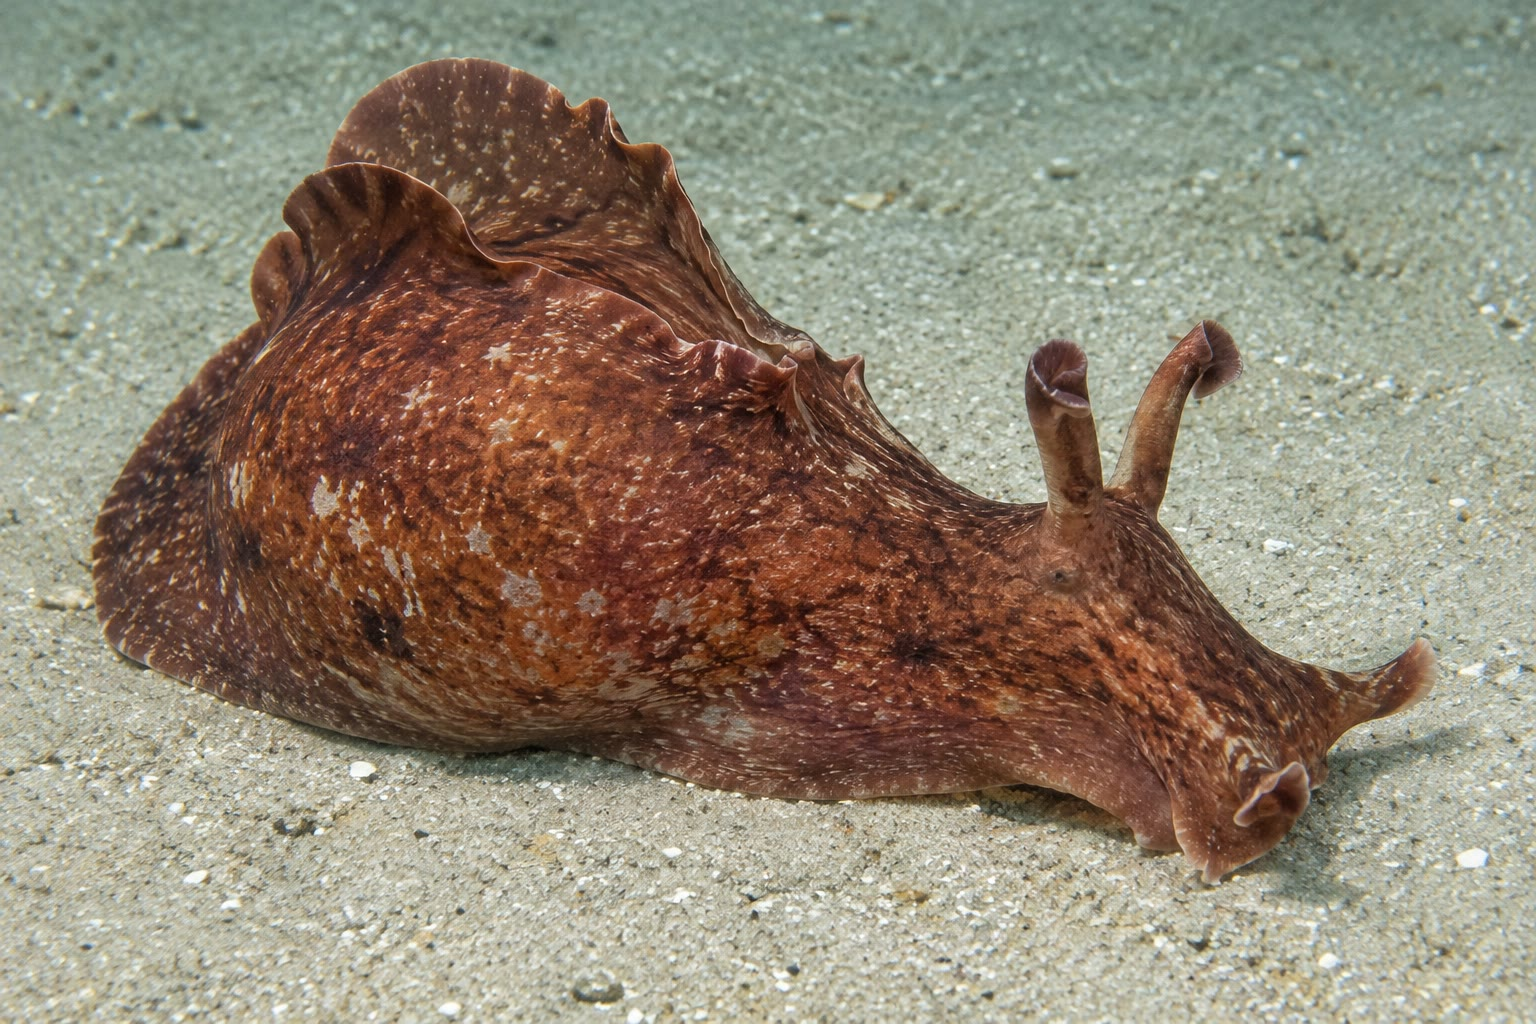
\includegraphics[width=0.46\linewidth]{images/book5/ai/b5-19-aplysia.jpg}\hspace{0.04\linewidth}
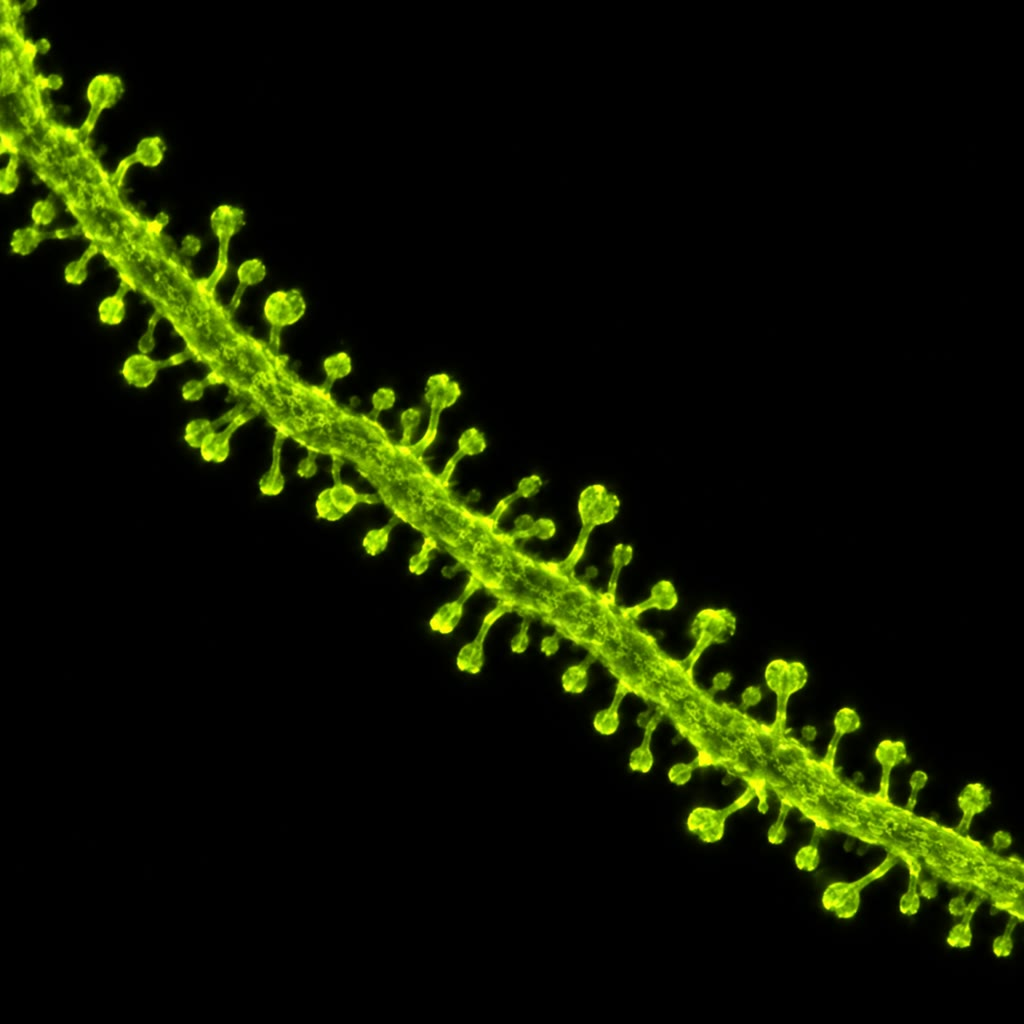
\includegraphics[width=0.36\linewidth]{images/book5/ai/b5-19-dendritic-spines.jpg}

{\small يسارًا: \emph{Aplysia californica}، التي تتيح
عصبوناتها القليلة الكبيرة إيجاد مشبك ذكرى وتسجيله. ويمينًا:
تغصن مرصَّع بالشوكات، كل واحدة الجانب بعد المشبكي لمشبك
مهيِّج واحد وكل واحدة حجيرة يقرر كالسيومها مصيرها هي.}
\end{omfigure}

\section{دارات للأماكن والأحداث}

\begin{definition}[دارة الحُصين]\label{def:b3:learning-memory:hippocampus}
\index{تلفيف مسنن}\index{CA3}\index{CA1}\index{خلية مكان}\index{خلية شبكية}\index{إتمام النمط}\index{إعادة}
يبلغ الدخل القشري الحُصينَ عبر القشرة الأنفية الباطنة ويمر
بثلاث مراحل: \emph{التلفيف المسنن}، الذي تفوق خلاياه
الحبيبية دخلاته عددًا وتشتعل تناثرًا (ففصل الأنماط
المتشابهة)؛ و\emph{CA3}، الذي تتصل خلاياه الهرمية بعضها
ببعض اتصالًا راجعًا، وكل واحدة تتلقى آلاف المشابك من غيرها
--- أي شبكة \emph{ترابطية ذاتية} تقدر على إتمام نمط مخزون
من شظية منه؛ و\emph{CA1}، الذي يقارن خرج CA3 بالدخل المباشر
ويعيد النتيجة إلى القشرة. وفي جرذ يستكشف ساحة، لا تشتعل
خلية هرمية حُصينية إلا حين يكون الحيوان في مكان واحد ---
وهي \emph{خلية المكان} (أوكيف، 1971) --- وبضع مئات منها ترسم
الساحة؛ وفي القشرة الأنفية الباطنة قبلها، تشتعل \emph{الخلايا
\omterm{def:b3:sensory-systems:retina}{الشبكية}} (موزر، 2005) عند رؤوس شبكة سداسية تغطي الفضاء، وهي
جملة إحداثيات تُبنى منها حقول الأماكن. وأثناء النوم والراحة
\emph{تُعاد} متواليات خلايا المكان التي اشتعلت أثناء الركض
بسرعة عالية، وحجب الإعادة يضعف ذاكرة الركضة: \omterm{def:b3:learning-memory:kinds}{فالحُصين} يكرر
دروب النهار على القشرة.
\end{definition}

\begin{omfigure}
\begin{tikzpicture}[every node/.style={font=\scriptsize}, >=stealth]
  % trisynaptic loop
  \node[draw, thick, rounded corners, fill=gray!15, align=center] (ec) at (0,0) {القشرة الأنفية الباطنة\\(خلايا شبكية)};
  \node[draw, thick, rounded corners, fill=omDef!20, align=center] (dg) at (3.2,1.4) {التلفيف المسنن:\\فصل الأنماط};
  \node[draw, thick, rounded corners, fill=omProp!30, align=center] (ca3) at (7.2,1.4) {CA3، راجع:\\إتمام النمط};
  \node[draw, thick, rounded corners, fill=omMeth!25, align=center] (ca1) at (7.2,-1.4) {CA1:\\يقارن ويُخرج};
  \draw[->, thick] (ec) -- (dg); \draw[->, thick] (dg) -- (ca3); \draw[->, thick] (ca3) -- (ca1); \draw[->, thick] (ca1) -- (ec) node[pos=0.3, below, sloped, font=\tiny] {رجوع إلى القشرة};
  \draw[->, thick, dashed] (ec) -- (ca1.north west) node[pos=0.7, above, sloped, font=\tiny] {السبيل المباشر};
  \draw[->, thick, omProp!80!black] (ca3.north) .. controls (6.6,2.6) and (7.8,2.6) .. (ca3.north east) node[pos=0.5, above, font=\tiny] {فروع راجعة};
  % place field map
  \begin{scope}[xshift=10.4cm, yshift=-0.2cm]
    \draw[thick] (0,0) rectangle (3,2.4); \node[below] at (1.5,-0.05) {الساحة، من فوق};
    \foreach \p/\c in {(0.7,1.8)/omThm, (2.1,1.9)/omDef, (1.4,0.9)/omMeth, (2.5,0.6)/omProp} { \fill[\c!60] \p circle (0.32); \fill[\c!90] \p circle (0.16); }
    \node[above] at (1.5,2.45) {حقول اشتعال أربع خلايا مكان};
  \end{scope}
\end{tikzpicture}

{\small يسارًا: عروة \omterm{def:b3:learning-memory:kinds}{الحُصين} --- فصل في \omterm{def:b3:learning-memory:hippocampus}{التلفيف المسنن}، وتخزين
وإتمام في \omterm{def:b3:learning-memory:hippocampus}{CA3} الراجع، ومقارنة في \omterm{def:b3:learning-memory:hippocampus}{CA1}. ويمينًا: كل \omterm{def:b3:learning-memory:hippocampus}{خلية مكان}
تشتعل في منطقة واحدة من الساحة؛ وهي معًا ترسم الفضاء.}
\end{omfigure}

\begin{proposition}[كم تسع شبكة ترابطية ذاتية]\label{prop:b3:learning-memory:capacity}
\index{شبكة هوبفيلد}\index{سعة الذاكرة}
شبكة من $N$ عصبونًا، كل واحد موصول بالبقية بأوزان هِبّية
$w_{ij} \propto \sum_{\mu}\xi_{i}^{\mu}\xi_{j}^{\mu}$ مجموعة
على الأنماط الثنائية المخزونة $\xi^{\mu}$، تستعيد نمطًا
مخزونًا من إشارة مشوَّهة أو جزئية باستقرارها فيه جاذبًا
(هوبفيلد، 1982). وهي تفعل ذلك على نحو موثوق حتى نحو $P
\approx 0.14N$ نمط عشوائي؛ وبعد ذلك تتداخل الأنماط وينهار
الاسترجاع. \omterm{def:b3:learning-memory:hippocampus}{وCA3} عند الجرذ، وفيه نحو $3\times 10^{5}$ خلية
هرمية، قد يسع بهذا التقدير نحو $4\times 10^{4}$ نمط ---
وهو من رتبة عدد الأماكن أو الحوادث المتمايزة التي يلقاها
حيوان في موسم --- ويرفع اشتعاله المتناثر (بضع في المئة من
الخلايا فعالة في أي نمط) السعة أكثر. \omterm{def:b3:learning-memory:hippocampus}{وإتمام النمط} من إشارة
هو ما يجعل رائحةً أو ركنًا يستدعي مشهدًا كاملًا؛ وثمنه أن
الذكريات المتشابهة تندمج، وهو ما يقاومه فصل \omterm{def:b3:learning-memory:hippocampus}{التلفيف المسنن}.
\end{proposition}
\admitted

\begin{method}[اختبار الذاكرة وآليتها]\label{met:b3:learning-memory:tests}
\index{متاهة موريس المائية}\index{إشراط الخوف}\index{أثر ذاكري}
(1) مهمة مكانية: \omterm{met:b3:learning-memory:tests}{متاهة موريس المائية} --- يسبح جرذ في ماء
عكر إلى منصة مخبأة في موضع ثابت، فيتعلم موضعها من إشارات
الغرفة على مدى أيام، ويُختبر بالزمن الذي يقضيه باحثًا في
الربع الصحيح حين تُزال المنصة؛ وآفات \omterm{def:b3:learning-memory:kinds}{الحُصين}، وحاجبات NMDA،
وفقد \omterm{def:b3:learning-memory:ltp}{التقوية طويلة الأمد} يلغي كل منها التعلم. (2) مهمة
ترابطية: \omterm{def:b3:learning-memory:kinds}{الإشراط} الخوفي --- نغمة تقترن بصدمة في القدم تصير
مستدعية للتجمد؛ وتتوقف الذكرى على اللوزة، وتتوقف صورة
نوعية السياق منها على \omterm{def:b3:learning-memory:kinds}{الحُصين}. (3) اختبار آلية: احجب
المرشَّح (بدواء، أو \omterm{def:b3:genetic-engineering:transgenic}{بحذف مورّثي} محصور في منطقة وزمن) وبيّن
أن التعلم يخفق بينما لا يخفق الإدراك ولا الحركة. (4) \omterm{met:b3:learning-memory:tests}{الأثر
الذاكري}: وسِم العصبونات الفعالة أثناء التعلم بقناة حساسة
للضوء (\cref{ch:b3:nervous-systems}) ثم أعد تفعيلها لاحقًا
بالضوء --- فيتجمد الحيوان في سياق آمن، كأنه يتذكر؛ وإسكاتها
يحجب الاسترجاع. فالذاكرة في خلايا يمكن تعيينها وفي مشابكها،
ويمكن تشغيلها وإطفاؤها.
\end{method}

\begin{omfigure}
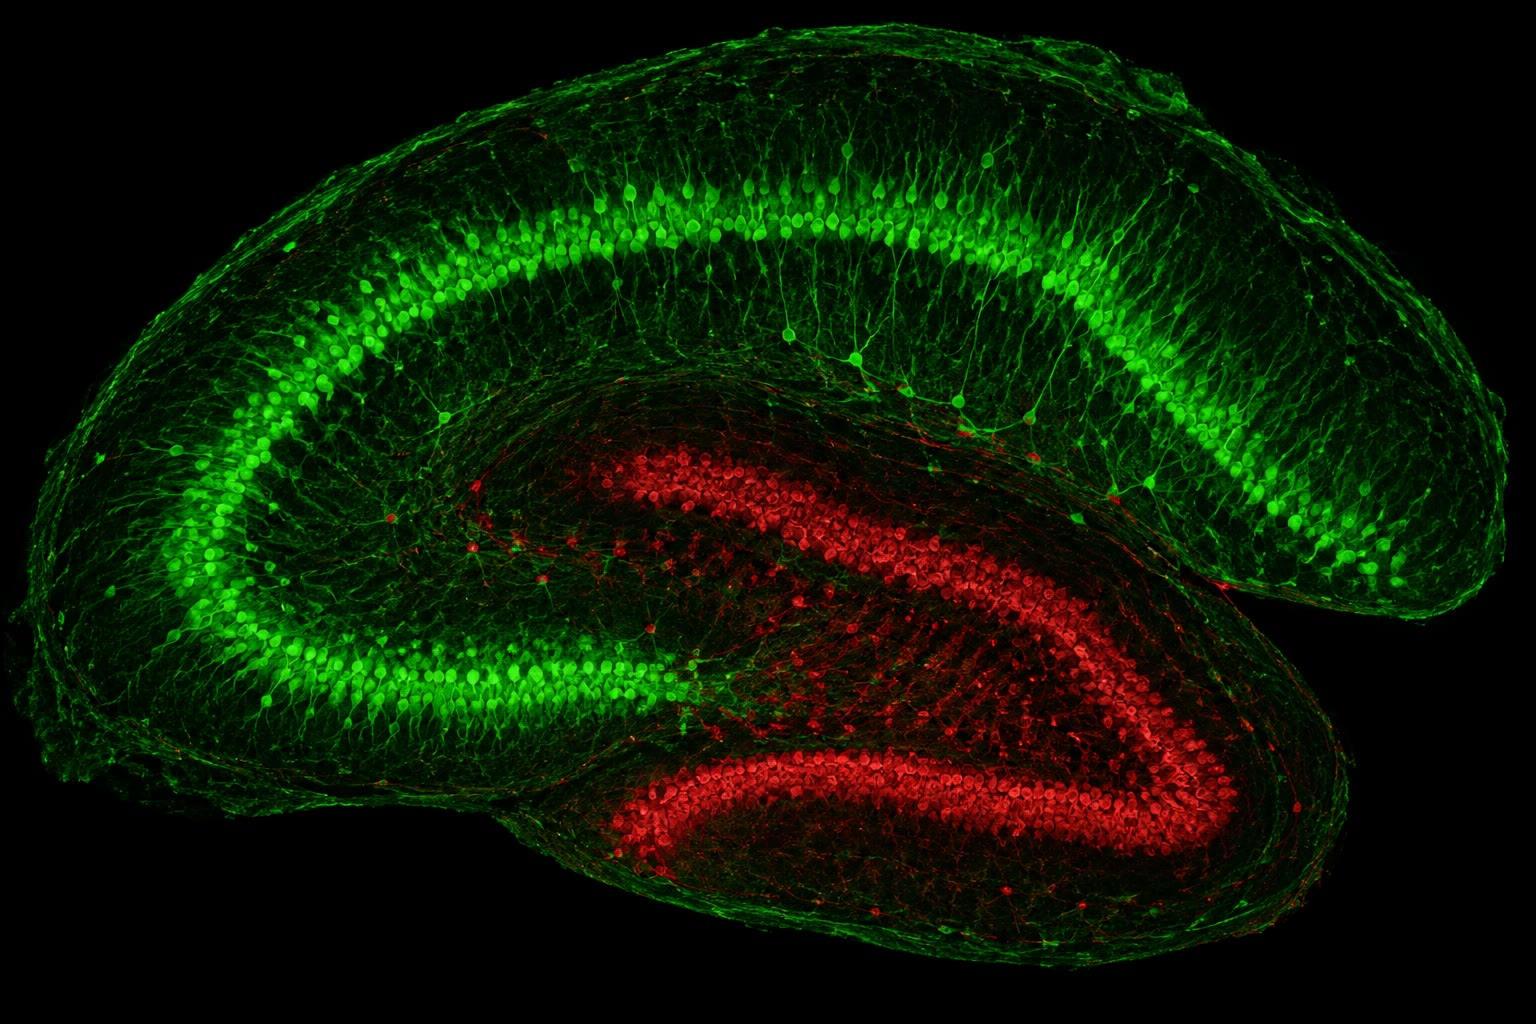
\includegraphics[width=0.56\linewidth]{images/book5/ai/b5-19-hippocampus-section.jpg}

{\small مقطع في \omterm{def:b3:learning-memory:kinds}{حُصين} قارض: الشريط المنحني من الخلايا
الهرمية (بالأخضر) من \omterm{def:b3:learning-memory:hippocampus}{CA3} إلى \omterm{def:b3:learning-memory:hippocampus}{CA1} \omterm{def:b3:learning-memory:hippocampus}{والتلفيف المسنن} المتشابك
معه (بالأحمر). وكل ذكرى مكانية عند الحيوان تمر بهذه العروة.}
\end{omfigure}

\section{المكافأة، والتنبؤ، ولدونة العمر كله}

\begin{proposition}[التعلم بخطأ التنبؤ]\label{prop:b3:learning-memory:rescorla}
\index{قاعدة ريسكورلا--واغنر}\index{خطأ التنبؤ}\index{دوبامين}
ليكن $V$ القيمة التي يعلّقها حيوان على إشارة وليكن $\lambda$
المكافأة التي تتلوها. \omterm{prop:b3:learning-memory:rescorla}{فقاعدة ريسكورلا--واغنر} (1972) تقول إن
القيمة تتغير في كل محاولة بكسر $\alpha$ من \emph{\omterm{prop:b3:learning-memory:rescorla}{خطأ
التنبؤ}}:
\[
\Delta V = \alpha\,(\lambda - V), \qquad
V_{n} = \lambda\bigl(1 - (1-\alpha)^{n}\bigr) ,
\]
فالتعلم سريع في البداية ويبطؤ مع تحسن التنبؤ، ويتوقف حين
تصير المكافأة متنبَّأً بها تمامًا، وينعكس (الانطفاء) حين
تُمنع المكافأة. وحين تُعرض إشارتان معًا تتشاركان تنبؤًا
واحدًا، فالإشارة التي لا تضيف شيئًا إلى تنبؤ قائم لا
تُتعلَّم (\emph{الحجب}). وسجّل شولتز (1997) من عصبونات
الدوبامين في الدماغ المتوسط عند قردة فوجد أنها تشتعل
لمكافأة غير متوقعة، وتصمت لمكافأة متنبَّأ بها تمامًا، وتهبط
دون خط الأساس حين تخفق مكافأة متوقعة في الوصول: فهي تبث
$\lambda - V$، أي \omterm{prop:b3:learning-memory:rescorla}{خطأ التنبؤ} نفسه، إلى المخطط والقشرة، حيث
يبوّب الدوبامين اللدونة عند المشابك التي كانت فعالة حديثًا.
فتعلم ما يتنبأ بالمكافأة لدونةٌ هِبّية بعامل ثالث يقول هل
كانت النتيجة أفضل أم أسوأ مما كان متوقعًا --- وأما عقاقير
\omterm{def:b3:learning-memory:critical}{الإدمان}، بسوقها الدوبامين مباشرةً، فتزوّر ``أفضل مما توقعت''
دائمة.
\end{proposition}
\begin{proof}
التراجع $V_{n+1} = V_{n} + \alpha(\lambda - V_{n})$ يعطي
$\lambda - V_{n+1} = (1-\alpha)(\lambda - V_{n})$، فيتقلص الخطأ
تقلصًا هندسيًا، $\lambda - V_{n} = (1-\alpha)^{n}\lambda$ من $V_{0} =
0$، ومنه الصيغة. وأما لإشارتين $A$ و$B$ تُعرضان معًا
فالتنبؤ هو $V_{A} + V_{B}$؛ فإذا دُرّبت $A$ أولًا حتى
$V_{A} = \lambda$، كان الخطأ في المحاولات المركّبة صفرًا ولم
تكتسب $B$ شيئًا.
\end{proof}

\begin{omfigure}
\begin{tikzpicture}
\begin{axis}[
  width=6.6cm, height=5.0cm,
  axis x line=bottom, axis y line=left,
  xmin=0, xmax=25, ymin=0, ymax=1.1,
  xlabel={المحاولة $n$}, ylabel={$V_{n}/\lambda$},
  xlabel style={font=\small, at={(axis description cs:0.5,-0.14)}, anchor=north}, ylabel style={font=\small},
  tick label style={font=\scriptsize}, xtick={0,5,10,15,20,25}, ytick={0,0.5,1},
  clip=false,
]
\addplot[very thick, omDef, domain=0:12, samples=13] {1-0.8^x};
\addplot[very thick, omDef, domain=12:25, samples=14] {(1-0.8^12)*0.8^(x-12)};
\draw[dashed, gray] (axis cs:12,0) -- (axis cs:12,1.05);
\node[font=\scriptsize, anchor=north west, align=left] at (axis cs:0.5,0.98) {تُعطى المكافأة:\\اكتساب};
\node[font=\scriptsize, anchor=north west, align=left] at (axis cs:14,0.98) {تُمنع المكافأة:\\انطفاء};
\end{axis}
\begin{axis}[
  at={(7.6cm,0)}, anchor=south west,
  width=6.6cm, height=5.0cm,
  ybar, bar width=14pt,
  axis x line=bottom, axis y line=left,
  ymin=-1.2, ymax=1.5,
  symbolic x coords={unexpected reward, predicted reward, reward omitted},
  xticklabels={مكافأة غير متوقعة, مكافأة متنبَّأ بها, مكافأة محذوفة},
  xtick=data, ytick={-1,0,1}, yticklabels={هبوط,خط الأساس,دفقة},
  ylabel={اشتعال الدوبامين},
  x tick label style={font=\scriptsize, align=center, text width=1.9cm}, ylabel style={font=\small}, tick label style={font=\scriptsize},
  clip=false,
]
\addplot[fill=omThm!50, draw=omThm] coordinates {(unexpected reward,1.2) (predicted reward,0.05) (reward omitted,-1.0)};
\end{axis}
\end{tikzpicture}

{\small يسارًا: منحنى تعلم ريسكورلا--واغنر عند $\alpha = 0.2$
--- اقتراب هندسي من قيمة المكافأة، ثم انطفاء حين تتوقف
المكافأة. ويمينًا: عصبونات الدوبامين تخبر \omterm{prop:b3:learning-memory:rescorla}{بخطأ التنبؤ} ---
دفقة للمفاجأة، ولا شيء لمكافأة متنبَّأ بها، وهبوط حين تفوت
مكافأة متوقعة.}
\end{omfigure}

\begin{definition}[الفترات الحرجة وأمراض اللدونة]\label{def:b3:learning-memory:critical}
\index{فترة حرجة}\index{سيادة عينية}\index{إدمان}\index{داء ألزهايمر}
اللدونة أعظم ما تكون في نوافذ من النماء. فقد غطّى هيوبل
وويزل (في ستينيات القرن العشرين) إحدى عيني هريرة بضعة أسابيع
بعد الولادة: فصارت القشرة البصرية، التي تسوقها العينان
عادةً في أعمدة متناوبة، مسوقة كلها تقريبًا بالعين المفتوحة،
وبقيت العين المحرومة عمياء وظيفيًا مدى الحياة --- بينما لم
يغيّر الحرمان نفسه شيئًا في قط بالغ. وهذه \emph{الفترات
الحرجة}، للبصر، وللغة، ولأغاني الطيور، تُغلق حين تنضج
الدارات المثبِّطة ويتصلّب المهد خارج الخلوي، ويمكن فتحها
قليلًا بالأدوية والتدريب. وأمراض اللدونة أمراض جرعة وهدف:
فإن \emph{الإدمان} تعلمٌ يسوقه خطأ تنبؤ مزوَّر، فيبني عادات
تعمّر أطول من اللذة؛ وكرب ما بعد الصدمة ذكرى خوف فرطت
هرمونات الشدة في ترسيخها؛ و\emph{داء ألزهايمر} يبدأ حيث
تبدأ \omterm{def:b3:learning-memory:kinds}{الذاكرة التصريحية}، في القشرة الأنفية الباطنة \omterm{def:b3:learning-memory:kinds}{والحُصين}،
بفقد المشابك --- وهو يتابع الخرف أفضل من أي عدّ للّويحات
--- قبل فقد العصبونات.
\end{definition}

\begin{remark}[مِمَّ تُصنع الذاكرة]\label{rem:b3:learning-memory:what}
الذكرى ليست تسجيلًا بل تغيّرًا في قوى المشابك وأعدادها،
موزَّعًا على الخلايا التي كانت فعالة حين صُنعت، موضوعًا
بقاعدة تقوّي ما يشتعل معًا، مبوَّبًا بإشارة تقول هل كانت
النتيجة مهمة، ومكرَّرًا في النوم حتى تحفظه القشرة وحدها.
فالقاعدة \omterm{def:b3:learning-memory:ltp}{قاعدة هِب}، والبوابة \omterm{prop:b3:learning-memory:nmda}{مستقبل NMDA}، والإشارة
الدوبامين، والتكرار هو \omterm{def:b3:learning-memory:hippocampus}{الإعادة}، والرياضيات تقول ما يسع جهاز
كهذا ولماذا يخلط بين المتشابهات. وكل تجربة شغّلت ذكرى أو
أطفأتها --- بحاجب، أو بمورّثة، أو بضوء --- وجدتها في تلك
المشابك، في تلك الخلايا. ومات H.M. عام 2008؛ ودماغه، وقد
قُطّع وصُوّر، أظهر الآفة التي علّمت الحقل، ولا شيء أكثر.
\end{remark}

\section{تمارين}

\begin{exercise}[$\star$]\label{exo:b3:learning-memory:1}
ميّز \omterm{def:b3:learning-memory:kinds}{الذاكرة التصريحية} من غير التصريحية بأداء H.M.، وسمّ
منطقة دماغية لكل ضرب من أربعة أضرب من الذاكرة غير
التصريحية.
\end{exercise}

\begin{exercise}[$\star$]\label{exo:b3:learning-memory:2}
اذكر مصادرة هِب والخصائص الثلاث \omterm{def:b3:learning-memory:ltp}{للتقوية طويلة الأمد} التي
تتبع منها.
\end{exercise}

\begin{exercise}[$\star$]\label{exo:b3:learning-memory:3}
اشرح لماذا يكون \omterm{prop:b3:learning-memory:nmda}{مستقبل NMDA} كاشفًا للتزامن، وماذا يحدث
\omterm{def:b3:learning-memory:ltp}{للتقوية طويلة الأمد} حين يُطبَّق حاجبه AP5 قبل الكزاز، وبعده.
\end{exercise}

\begin{exercise}[$\star$]\label{exo:b3:learning-memory:4}
في \emph{Aplysia}، ما الذي يميّز \omterm{def:b3:learning-memory:kinds}{التحسيس} القصير الأمد من
الطويل الأمد على المستوى الجزيئي، وأي تجربة تبيّن ذلك؟
\end{exercise}

\begin{exercise}[$\star\star$]\label{exo:b3:learning-memory:5}
عند $\alpha = 0.3$، كم محاولة حتى تبلغ $V$ نسبة \qty{90}{\%} من
$\lambda$؟ وإذا مُنعت المكافأة عندئذ، كم محاولة حتى تهبط $V$
دون \qty{10}{\%}؟ ولماذا يكون الاكتساب والانطفاء متناظرين في
هذا النموذج، وهل هما كذلك في الحيوانات؟
\end{exercise}

\begin{exercise}[$\star\star$]\label{exo:b3:learning-memory:6}
دخلان عندهما $C = \begin{pmatrix}1 & 0.5\\ 0.5 & 1\end{pmatrix}$.
جِد المتجهات الذاتية والقيم الذاتية، وقل نحو أي اتجاه تدير
\omterm{def:b3:learning-memory:ltp}{قاعدة هِب} الأوزان وماذا يكشف العصبون عندئذ. وطبّق \omterm{thm:b3:learning-memory:hebb}{قاعدة
أويا} خطوةً واحدة من $\mathbf{w} = (1,0)$ عند دخل $\mathbf{x}
= (1,1)$ و$\eta = 0.1$.
\end{exercise}

\begin{exercise}[$\star\star$]\label{exo:b3:learning-memory:7}
حجم شوكة \qty{0.1}{fL}. فدخول $500$ أيون كالسيوم يرفع تركيزه
الحر بكم (بوحدة $\unit{\micro mol/L}$)، إذا ارتبط
\qty{95}{\%} منها فورًا بالموقيات؟ وقارن ذلك بمستوى الراحة
\qty{0.1}{\micro mol/L} وبالثابت $K_{d}$ للكالمودولين مفعِّل
CaMKII، وهو نحو \qty{1}{\micro mol/L}.
\end{exercise}

\begin{exercise}[$\star\star$]\label{exo:b3:learning-memory:8}
اشرح الحجب \omterm{prop:b3:learning-memory:rescorla}{بقاعدة ريسكورلا--واغنر} واذكر تسجيل الدوبامين
الموافق لكل مرحلة.
\end{exercise}

\begin{exercise}[$\star\star$]\label{exo:b3:learning-memory:9}
تنبأ بنتائج (أ) حذف \omterm{prop:b3:learning-memory:nmda}{مستقبل NMDA} محصورًا في \omterm{def:b3:learning-memory:hippocampus}{CA1}، و(ب) مثبط
لتركيب البروتين يُعطى أثناء التدريب، و(ج) المثبط نفسه يُعطى
بعد يوم، و(د) \omterm{def:b3:learning-memory:hippocampus}{إعادة} تفعيل ضوئية وراثية لخلايا \omterm{def:b3:learning-memory:hippocampus}{التلفيف
المسنن} التي كانت فعالة أثناء \omterm{def:b3:learning-memory:kinds}{إشراط} خوفي، في سياق جديد.
\end{exercise}

\begin{exercise}[$\star\star\star$]\label{exo:b3:learning-memory:10}
بيّن أنه \omterm{def:b3:learning-memory:ltp}{بقاعدة هِب} وحدها ينمو طول $\mathbf{w}$ بلا حد، وأن
\omterm{thm:b3:learning-memory:hebb}{قاعدة أويا} تعطي $|\mathbf{w}| = 1$ عند أي نقطة ثابتة. ولماذا
يكون النمو غير المحدود مشكلة بيولوجية، وأي الآليات (التحجيم
المشبكي، \omterm{def:b3:learning-memory:ltp}{والاكتئاب طويل الأمد}، والنوم) قد توافق الحدَّ
المعيِّر؟
\end{exercise}

\begin{exercise}[$\star\star\star$]\label{exo:b3:learning-memory:11}
في \omterm{def:b3:learning-memory:hippocampus}{CA3} عند الجرذ $3\times 10^{5}$ خلية؛ وعند الإنسان نحو $2\times 10^{6}$.
قدّر سعة هوبفيلد لكل منهما. ولماذا يكون التقدير مقياسًا
رديئًا لعدد الذكريات التي يحفظها إنسان، وماذا يضيف دور
\omterm{def:b3:learning-memory:kinds}{الحُصين} في \omterm{def:b3:learning-memory:kinds}{الترسيخ} إلى الصورة؟
\end{exercise}

\begin{exercise}[$\star\star\star$]\label{exo:b3:learning-memory:12}
الهريرات المحرومة من إبصار إحدى العينين أسابيع تفقد إقليم
تلك العين القشري؛ والبوالغ لا تفقده. اشرح بالتنافس الهِبّي
لماذا تفوز العين المفتوحة، ولماذا يكون أثر حرمان العينين
أصغر من حرمان واحدة، وما الذي يغلق \omterm{def:b3:learning-memory:critical}{الفترة الحرجة}.
\end{exercise}

\section{مسألة: مشبك يتذكر}

\begin{problem}[{مسألة نهاية الأسبوع --- ذكرى تُتبَّع من كالسيوم
في شوكة إلى جرذ في متاهة: حساب الكالسيوم في الاستحداث،
وعصبون هِبّي يتقارب إلى ما تشترك فيه دخلاته، ومنحنى تعلم
يوقّته خطأ التنبؤ، وسعة حُصين، وتُختم بتركيز الكالسيوم الذي
يستحدث التقوية، وبالمحاولات التي يحتاج إليها جرذ، وبالأنماط
التي يسعها CA3 عنده}]
\label{pb:b3:learning-memory:1}
المعطيات: شوكة حجمها \qty{0.08}{fL}؛ وكل قناة NMDA تحمل
$10^{3}$ من Ca$^{2+}$ في كل انفتاح مدته \qty{50}{ms}؛ وللمشبك
$10$ مستقبلات NMDA؛ ويُوقَّى \qty{98}{\%} من الكالسيوم
الداخل؛ والكالسيوم الحر في الراحة \qty{0.1}{\micro mol/L}؛
ويُفعَّل CaMKII فوق \qty{2}{\micro mol/L} من الكالسيوم الحر،
والكالسينورين بين $0.3$ و\qty{1}{\micro mol/L}. وهِب: دخلان
عند $C = \begin{pmatrix}1 &
0.6\\ 0.6 & 1\end{pmatrix}$، و$\eta = 0.1$. وريسكورلا--واغنر: $\alpha =
0.15$. والسعة: \omterm{def:b3:learning-memory:hippocampus}{CA3} عند الجرذ $3\times 10^{5}$ خلية، و$P = 0.14N$؛
والجرذ يستكشف $20$ مكانًا جديدًا في اليوم.

\medskip
\noindent\textbf{الجزء الأول --- الكالسيوم.}
\begin{enumerate}
  \item تنفتح مستقبلات NMDA العشرة كلها مرة واحدة. فكم أيون
        كالسيوم يدخل، وكم يبقى حرًّا، وأي ارتفاع في التركيز
        ذلك في الشوكة؟
  \item هل يُفعَّل CaMKII؟ وماذا لو لم ينفتح إلا مستقبلان
        (أُطلق الغلوتامات ولم يكد يزول استقطاب الشوكة)؟
  \item مع انفتاح مستقبلين، أي إنزيم يقع في مداه، وماذا يحدث
        للمشبك؟ واشرح كيف يقدر أيون واحد على إنتاج التقوية
        والاكتئاب معًا.
  \item يُضخ الكالسيوم إلى الخارج بثابت زمن قدره \qty{20}{ms}.
        فلماذا يجب أن تصل الدخلات في غضون عشرات الميلي ثانية
        لتجمع كالسيومها، وكيف يحدد ذلك نافذة توقيت الشوكات؟
  \item تبعد شوكة \qty{0.5}{\micro m} عن جارتها على التغصن.
        اشرح لماذا يبقي التوقي وعنق الشوكة الضيق إشارة
        الكالسيوم في شوكة واحدة، ولماذا يهم ذلك في نوعية
        الدخل.
  \item يُرفع حجب المغنيزيوم عند نحو \qty{-30}{mV}. ومشبك AMPA
        واحد يزيل استقطاب الشوكة \qty{5}{mV} من \qty{-70}{mV}.
        فكم دخلًا متزامنًا (أو ماذا غير ذلك) يلزم لفك حجب
        مستقبلات NMDA؟ وماذا يقول ذلك عن التعاون؟
\end{enumerate}

\medskip
\noindent\textbf{الجزء الثاني --- عصبون هِبّي.}
\begin{enumerate}[resume]
  \item جِد القيم الذاتية والمتجهات الذاتية للمصفوفة $C$.
  \item انطلاقًا من $\mathbf{w} = (1, 0)$، طبّق \omterm{def:b3:learning-memory:ltp}{قاعدة هِب}
        الوسطية $\mathbf{w} \leftarrow \mathbf{w} + \eta C\mathbf{w}$
        ثلاث خطوات. فما زاوية $\mathbf{w}$ إلى الاتجاه $(1,1)$
        بعد كل خطوة؟
  \item بعد خطوات كثيرة، ما النسبة $w_{2}/w_{1}$، وماذا يحدث
        للمقدار $|\mathbf{w}|$؟
  \item طبّق \omterm{thm:b3:learning-memory:hebb}{قاعدة أويا} الوسطية $\mathbf{w} \leftarrow \mathbf{w} +
        \eta\,(C\mathbf{w} - (\mathbf{w}^{\mathsf{T}}C\mathbf{w})
        \mathbf{w})$ خطوةً واحدة من $(0.8, 0.8)$. فنحو أي شيء
        تتحرك؟
  \item صار العصبون يستجيب للدخلين معًا. فإذا اشتعل الدخل 2
        وحده (وهو نادر)، ما مقدار $y$ بالنسبة إلى الحالة
        المشتركة، عند $\mathbf{w} = (0.71, 0.71)$؟
  \item اشرح في جملة واحدة كيف تكون ترابطية \omterm{def:b3:learning-memory:ltp}{التقوية طويلة
        الأمد} (أي تقوية دخل ضعيف مقترن بآخر قوي) هي هذه
        المبرهنة في العمل.
\end{enumerate}

\medskip
\noindent\textbf{الجزء الثالث --- منحنى التعلم.}
\begin{enumerate}[resume]
  \item عند $\alpha = 0.15$، احسب $V_{n}/\lambda$ بعد $5$ و$10$
        و$20$ محاولة.
  \item كم محاولة لبلوغ \qty{95}{\%} من $\lambda$؟
  \item يتعلم جرذ متاهة في نحو هذا العدد من المحاولات. فإذا
        ضوعفت المكافأة، هل يتنبأ النموذج بتعلم أسرع بالمحاولات؟
        وما الذي يتغير؟
  \item تُدرَّب الإشارة A حتى المقارب، ثم تُعرض A وB معًا
        بالمكافأة نفسها $20$ محاولة. فما $V_{B}$؟ وماذا تفعل
        عصبونات الدوبامين في المحاولات المركّبة؟
  \item صارت المكافأة تتلو B وحدها. صف \omterm{prop:b3:learning-memory:rescorla}{خطأ التنبؤ} واستجابة
        الدوبامين في المحاولة الأولى، ومسار $V_{B}$.
  \item دواء يرفع الدوبامين مهما تكن النتيجة. مستعملًا
        القاعدة، اشرح لماذا تُتعلَّم الأفعال السابقة للدواء
        كأنها كوفئت، مهما تكن عواقبها.
\end{enumerate}

\medskip
\noindent\textbf{الجزء الرابع --- \omterm{def:b3:learning-memory:kinds}{الحُصين}.}
\begin{enumerate}[resume]
  \item سعة هوبفيلد لمنطقة \omterm{def:b3:learning-memory:hippocampus}{CA3} عند الجرذ.
  \item عند $20$ مكانًا جديدًا في اليوم، كم يلزم قبل بلوغ
        السعة؟ وما الذي يجب أن يحدث ليواصل الحيوان التعلم؟
  \item ينقل \omterm{def:b3:learning-memory:kinds}{الترسيخ} الذكريات إلى القشرة على مدى أسابيع.
        اشرح لماذا يحمي النقل البطيء الذكريات القشرية القديمة
        (التداخل الكارثي) ولماذا يكون \omterm{def:b3:learning-memory:kinds}{الحُصين} مخزنًا مؤقتًا.
  \item إذا كانت \qty{3}{\%} من خلايا \omterm{def:b3:learning-memory:hippocampus}{CA3} فعالة في أي نمط، فكم
        خلية ترمّز مكانًا واحدًا، وكم نمطًا يمكن تمييزه لو
        اشتُرط ألا تتشارك الأنماط أكثر من نصف خلاياها؟ (احتجّ
        نوعيًا لماذا يرفع الترميز المتناثر السعة.)
  \item تضغط \omterm{def:b3:learning-memory:hippocampus}{الإعادة} أثناء النوم ركضة مدتها \qty{10}{s} إلى
        \qty{0.5}{s}. فإذا كانت نافذة توقيت الشوكات
        \qty{20}{ms}، فأي تباعد بين اشتعالات خلايا المكان في
        الركضة يصير هِبّيًا في \omterm{def:b3:learning-memory:hippocampus}{الإعادة}؟ ولماذا قد يكون هذا هو
        مغزى الضغط؟
  \item تنجو ذكرى المتاهة من آفة حُصينية تُحدَث بعد شهر من
        التدريب لا من واحدة تُحدَث بعد يوم. فسّر ذلك، بنمط
        الفقد عند H.M.
  \item لخّص: تركيز الكالسيوم الحر بعد عشرة انفتاحات \omterm{prop:b3:learning-memory:nmda}{لمستقبل
        NMDA} (السؤال~1)، والمحاولات اللازمة لتعلم \qty{95}{\%}
        (السؤال~14)، وسعة \omterm{def:b3:learning-memory:hippocampus}{CA3} عند الجرذ (السؤال~19).
\end{enumerate}
\end{problem}
